

\section{virtual memory}

\subsection{address spaces}

\input{../vm/recallAddr}  % FIXME: some duplication with memProtect exceptions slides
\usetikzlibrary{arrows.meta,fit}

\begin{frame}{address spaces}
\begin{itemize}
\item illusion of \myemph{dedicated memory}
\end{itemize}
\myalttext{
\begin{tikzpicture}
\tikzset{
    every node/.style={font=\small},
}
\node[align=center] (progAAddr) {Process A \\ addresses};
\node[below=1cm of progAAddr,align=center] (progBAddr) {Process B \\ addresses};
\node[draw, right=3cm of progAAddr,align=center] (translationA) { mapping \\ (set by OS) };
\node[draw, right=3cm of progBAddr,align=center] (translationB) { mapping \\ (set by OS) };
\node[draw,rectangle split, rectangle split parts=6, anchor=north west,label={north:real memory}] (mem) at ([xshift=3.5cm]translationA.north east) {
    \nodepart{one}
    Process A code 
    \nodepart{two}
    Process B code
    \nodepart{three}
    Process A data
    \nodepart{four}
    Process B data
    \nodepart{five}
    OS data
    \nodepart{six}
    \ldots
};
\draw[-Latex,green,thick] (progAAddr) -- (translationA) (translationA.east) -- (mem.one west);
\draw[-Latex,green,thick] (translationA.east) -- (mem.three west);
\draw[-Latex,blue,thick] (progBAddr) -- (translationB) (translationB.east) -- (mem.two west);
\draw[-Latex,blue,thick] (translationB.east) -- (mem.four west);
\node[thick,draw,anchor=north west] (error) at ([yshift=-.5cm]mem.south west) {trigger exception};
\draw[-Latex,green,thick] (translationA.east) -- (error.west);
\draw[-Latex,blue,thick] (translationB.east) -- (error.west);
\draw[-Latex,green,ultra thick,dotted] (translationA.east) -- (mem.five west);
\draw[-Latex,blue,ultra thick,dotted] (translationB.east) -- (mem.five west);
\draw[-Latex,ultra thick,dotted] ([xshift=-3cm,yshift=-.5cm]translationB.south) -- ([xshift=-2cm,yshift=-.5cm]translationB.south)
    node[right] {= kernel-mode only};
\begin{visibleenv}<2>
    \node[fill=red,fill opacity=0.1,draw=red,ultra thick,fit=(translationA) (translationB),label={[red]north:chose one during context switch}] {};
\end{visibleenv}
\end{tikzpicture}
}{Diagram showing processes A and B have different mappings from virtual (program) to physical (real) addresses set by the OS.
The mapping can also specifies that some addresses trigger exceptions or are usable in kernel mode only.}
\end{frame}


\subsection{address translation overview}
\input{../vm/translationOverview}

\subsection{simple paging with four pages}
\input{../vm/fourPages}

\subsection{on address space sizes}
\input{../vm/sizeNotes}

\subsection{exercise: address splitting}
\input{../vm/ptSizeEx}

\subsection{exercise: simple lookup}
\begin{frame}{exercise: page table lookup}
    \begin{itemize}
    \item suppose 64-byte pages (= 6-bit page offsets), 9-bit virtual addresses
    \end{itemize}
\begin{tabular}{l|l|l}
VPN & valid & PPN \\ \hline
\tt 000 & \tt 1 & \tt 0010 \\ \hline
\tt 001 & \tt 1 & \tt 1010 \\ \hline
\tt 010 & \tt 0 & \tt --- \\ \hline
\tt 011 & \tt 0 & \tt --- \\ \hline
\tt 100 & \tt 1 & \tt 1110 \\ \hline
\tt 101 & \tt 1 & \tt 0100 \\ \hline
\tt 110 & \tt 1 & \tt 0001 \\ \hline
\tt 111 & \tt 0 & \tt --- \\ \hline
\end{tabular}
    \begin{itemize}
    \item virtual address {\tt 0x024} ({\tt 0 0010 0100}) = physical address ???
    \end{itemize}
\end{frame}


\section{permissions in page tables}
\subsection{read-only}
\usetikzlibrary{calc,patterns,positioning}

\begin{frame}[label=progMem]{vim (two copies)}
\begin{tikzpicture}
\tikzset{
    mylabel/.style={font=\ttfamily},
    mybox/.style={draw,rectangle,minimum width=7cm,fill=white,inner sep=1mm},
    myhigh/.style={draw,rectangle,line width=1mm, draw=blue!80!black,opacity=.3},
}
\begin{scope}[name prefix=A-]
\node[mybox,minimum height=1cm,pattern=north west lines,pattern color=black!5!white] (kernel) {Used by OS};
\node[above=0cm of kernel] {Vim (run by user mst3k)};
\node[mybox, minimum height=.5cm, below=1cm of kernel] (stack) {Stack};
\node[mybox, minimum height=.5cm, below=1cm of stack] (heap) {Heap / other dynamic};
\node[mybox, minimum height=.5cm, below=0mm of heap] (data) {Writable data};
\node[mybox, minimum height=.5cm, below=0mm of data] (sdata) {vim (Code + Constants)};
\coordinate (memBottom) at ($(sdata.south east) + (0mm, -2mm)$);
\begin{pgfonlayer}{bg}
\draw[pattern=north west lines, pattern color=black!40!white] (kernel.north west) rectangle (memBottom);
\end{pgfonlayer}
\end{scope}

\begin{scope}[name prefix=B-,xshift=8cm]
\node[mybox,minimum height=1cm,pattern=north west lines,pattern color=black!5!white] (kernel) {Used by OS};
\node[above=0cm of kernel] {Vim (run by user xyz4w)};
\node[mybox, minimum height=.6cm, below=1cm of kernel] (stack) {Stack};
\node[mybox, minimum height=1.4cm, below=.3cm of stack] (heap) {Heap / other dynamic};
\node[mybox, minimum height=.5cm, below=0mm of heap] (data) {Writable data};
\node[mybox, minimum height=.5cm, below=0mm of data] (sdata) {vim (Code + Constants)};
\coordinate (memBottom) at ($(sdata.south east) + (0mm, -2mm)$);
\begin{pgfonlayer}{bg}
\draw[pattern=north west lines, pattern color=black!40!white] (kernel.north west) rectangle (memBottom);
\end{pgfonlayer}
\end{scope}

\begin{visibleenv}<2->
\node[draw,red,ultra thick,inner sep=0.2mm,fit=(A-sdata) (B-sdata),label={[fill=white,fill opacity=0.8]south:\bf same data?}] {};  
\end{visibleenv}

\end{tikzpicture}
\end{frame}

\begin{frame}{two copies of program}
\begin{itemize}
\item would like to only have one copy of program
\vspace{.5cm}
\item what if {\tt mst3k}'s vim tries to modify its code?
\item would break process abstraction:
    \begin{itemize}
        \item ``illusion of own memory''
    \end{itemize}
\end{itemize}
\end{frame}
 % FIXME: move?

\subsection{permission bits}

\begin{frame}{permissions bits}
\begin{itemize}
\item page table entry will have more \myemph{permissions bits}
\begin{itemize}
\item can access in user mode?
\item can read from?
\item can write to?
\item can execute from?
\end{itemize}
\item checked by MMU like valid bit
\end{itemize}
\begin{tikzpicture}
\matrix[tight matrix,anchor=north west,
        nodes={text width=2.3cm,minimum height=0.3cm,font=\fontsize{10}{11}\selectfont\tt,black!80},
        column 1/.style={nodes={draw=none,align=right}},
        column 2/.style={nodes={draw,thick,text width=1.2cm,align=center}},
        column 3/.style={nodes={draw,thick,text width=1.2cm,align=center}},
        column 4/.style={nodes={draw,thick,text width=1.2cm,align=center}},
        column 5/.style={nodes={draw,thick,text width=1.2cm,align=center}},
        column 6/.style={nodes={draw,thick,text width=2.7cm}},
        row 1/.style={nodes={draw=none,font=\fontsize{10}{11}\selectfont\normalfont}},
        label={above:page table (logically)},
    ] (pt) at (0, 0) {
    virtual page \# \& valid? \& user? \& write? \& exec? \& physical page \# \\
    0000 0000 \& 0 \& 0 \& 0 \& 0 \& 00 0000 0000 \\
    0000 0001 \& 1 \& 1 \& 1 \& 0 \& 10 0010 0110\\
    0000 0010 \& 1 \& 1 \& 1 \& 0 \& 00 0000 1100 \\
    0000 0011 \& 1 \& 1 \& 0 \& 1 \& 11 0000 0011 \\
    \ldots \\
    1111 1111 \& 1 \& 0 \& 1 \& 0 \& 00 1110 1000 \\
};
\end{tikzpicture}
\end{frame}


\subsection{kernel-only}
\input{../vm/kernelOnly}

\section{page table tricks}
\subsection{space on demand}
\input{../vm/spaceOnDemand}

\subsection{switching address spaces}
\againframe<2>{progMemory}
\begin{frame}{running OS code}
    \begin{itemize}
    \item system calls, I/O events, etc. run OS code in kernel mode
    \vspace{.5cm}
    \item<2-> where in memory is this OS code?
        \begin{itemize}
            \item<3-> probably have a page table entry pointing to it
            \item<3-> marked not accessible in user mode
        \end{itemize}
    \item<4-> code better not be modified by user program
        \begin{itemize}
        \item otherwise: uncontrolled way to ``escape'' user mode
        \end{itemize}
    \end{itemize}
\end{frame}


\subsection{mmap}
\input{../vm/mmap}

\subsection{/proc/PID/maps}
\usetikzlibrary{arrows.meta,calc,matrix,shapes.misc}

\begin{frame}
\frametitle{Linux memory tracking}
\begin{itemize}
\item Linux kernel treats all program memory as special case of mmap'd file
\vspace{.5cm}
\item two major features to help
\item `private' mappings = copy-on-write from original file
    \begin{itemize}
    \item supports `load program from disk on demand'
    \item pages not shared with original file after writes
    \end{itemize}
\item original file = all zeroes (instead of file from disk)
    \begin{itemize}
    \item ``anonymous mapping''
    \item handles `allocate-on-demand' scenario
    \end{itemize}
\end{itemize}
\end{frame}

\begin{frame}[fragile,label=linuxMapsAreaStruct]{Linux maps: list of maps}
\lstset{language=}
\tikzset{
    btHLbox/.style={
        fill=red!30,outer sep=0pt,inner xsep=1pt, inner ysep=0pt, rounded corners=3pt
    },
}
\begin{lstlisting}[
    basicstyle=\fontsize{8.5}{9.5}\selectfont,
    moredelim={**[is][\btHL<1|handout:1>]{@2}{2@}},
    moredelim={**[is][\btHL<0|handout:0>]{@3}{3@}},
    moredelim={**[is][\btHL<0|handout:0>]{@4}{4@}},
    moredelim={**[is][\btHL<0|handout:0>]{@5}{5@}},
    moredelim={**[is][\btHL<0|handout:0>]{@6}{6@}},
    moredelim={**[is][\btHL<0|handout:0>]{@7}{7@}},
    moredelim={**[is][\btHL<0|handout:0>]{@8}{8@}},
]
$ cat /proc/self/maps
@200400000-0040b000 r-xp 00000000 08:01 48328831          /bin/cat2@
0060a000-0060b000 r--p 0000a000 08:01 48328831          /bin/cat
0060b000-0060c000 rw-p 0000b000 08:01 48328831          /bin/cat
01974000-01995000 rw-p 00000000 00:00 0                 [heap]
7f60c718b000-7f60c7490000 r--p 00000000 08:01 77483660  /usr/lib/locale/locale-archive
7f60c7490000-7f60c764e000 r-xp 00000000 08:01 96659129  /lib/x86_64-linux-gnu/libc-2.19.so
7f60c764e000-7f60c784e000 ---p 001be000 08:01 96659129  /lib/x86_64-linux-gnu/libc-2.19.so
7f60c784e000-7f60c7852000 r--p 001be000 08:01 96659129  /lib/x86_64-linux-gnu/libc-2.19.so
7f60c7852000-7f60c7854000 rw-p 001c2000 08:01 96659129  /lib/x86_64-linux-gnu/libc-2.19.so
7f60c7854000-7f60c7859000 rw-p 00000000 00:00 0 
7f60c7859000-7f60c787c000 r-xp 00000000 08:01 96659109  /lib/x86_64-linux-gnu/ld-2.19.so
7f60c7a39000-7f60c7a3b000 rw-p 00000000 00:00 0 
7f60c7a7a000-7f60c7a7b000 rw-p 00000000 00:00 0 
7f60c7a7b000-7f60c7a7c000 r--p 00022000 08:01 96659109  /lib/x86_64-linux-gnu/ld-2.19.so
7f60c7a7c000-7f60c7a7d000 rw-p 00023000 08:01 96659109  /lib/x86_64-linux-gnu/ld-2.19.so
7f60c7a7d000-7f60c7a7e000 rw-p 00000000 00:00 0 
7ffc5d2b2000-7ffc5d2d3000 rw-p 00000000 00:00 0         [stack]
7ffc5d3b0000-7ffc5d3b3000 r--p 00000000 00:00 0         [vvar]
7ffc5d3b3000-7ffc5d3b5000 r-xp 00000000 00:00 0         [vdso]
ffffffffff600000-ffffffffff601000 r-xp 00000000 00:00 0 [vsyscall]
\end{lstlisting}
\begin{tikzpicture}[overlay,remember picture]
    \begin{visibleenv}<2->
\node[fill=white,draw=red,ultra thick,anchor=south,align=left] at ([yshift=1cm]current page.south) {
OS tracks list of \texttt{struct vm\_area\_struct} with: \\
(shown in this output): \\
\hspace{.5cm}virtual address start, end \\
\hspace{.5cm}permissions \\
\hspace{.5cm}offset in backing file (if any) \\
\hspace{.5cm}pointer to backing file (if any) \\
~ \\
(not shown): \\
\hspace{.5cm}info about sharing of non-file data
\hspace{.5cm}\ldots
};
    \end{visibleenv}
\end{tikzpicture}
\end{frame}


\subsection{page table lookup}
\input{../vm/transEx} 

\subsection{aside: copy-on-write}
\input{../vm/copyOnWrite}

\subsection{fork with copy-on-write}
\input{../unix-api/fork-cow}

%\againframe<5>{forkPCBs}

\subsection{general page table tricks}
\begin{frame}{page tricks generally}
\begin{itemize}
\item deliberately \myemph{make program trigger page/protection fault}
\item but \myemph{don't assume page/protection fault is an error}
\vspace{.5cm}
\item have \myemph{seperate data structures} represent logically allocated memory
    \begin{itemize}
    \item e.g. ``addresses {\tt 0x7FFF8000} to {\tt 0x7FFFFFFFF} are the stack''
    \end{itemize}
\item page table is for the hardware and not the OS
\end{itemize}
\end{frame}

\begin{frame}{example page table tricks}
    \begin{itemize}
    \item allocating space on demand
    \item loading code/data from files on disk on demand
    \item copy-on-write
    \item \myemph<2>{saving data temporarily to disk, reloading to memory on demand}
        \begin{itemize}
        \item ``swapping''
        \end{itemize}
    \item \myemph<3>{detecting whether memory was read/written recently}
    \item \myemph<4>{stopping in a debugger when a variable is modified}
    \item \myemph<5>{sharing memory between programs on two different machines}
    \end{itemize}
\end{frame}

\begin{frame}{hardware help for page table tricks}
\begin{itemize}
\item information about the address causing the fault
    \begin{itemize}
    \item e.g. special register with memory address accessed
    \item harder alternative: OS disassembles instruction, look at registers
    \end{itemize}
\item (by default) rerun faulting instruction when returning from exception
\item precise exceptions: no side effects from faulting instruction or after
    \begin{itemize}
    \item e.g. {\tt pushq} that caused did not change {\tt \%rsp} before fault
    \item e.g. can't notice if instructions were executed in parallel
    \end{itemize}
\end{itemize}
\end{frame}


\subsection{page table in memory}
\input{../vm/ptInMemory}


\subsection{exercise: page table in memory}
\input{../vm/multiSplitExPt1}
\subsection{exercise (alt): page table in memory}
\input{../vm/multiSplitExPt1b}

\subsection{assignment preview 1}
\usetikzlibrary{matrix}
\begin{frame}{pagetable assignment}
    \begin{itemize}
    \item pagetable assignment
    \item simulate page tables (on top of normal program memory)
        \begin{itemize}
            \item alternately: implement another layer of page tables \\
                on top of the existing system's
        \end{itemize}
    \vspace{.5cm}
    \item in assignment:
    \item virtual address $\sim$ arguments to your functions
    \item physical address $\sim$ your program addresses (normal pointers)
    \end{itemize}
\end{frame}

\begin{frame}[fragile,label=asgnAPI]{pagetable assignment API}
\lstset{language=C,style=smaller}
\begin{lstlisting}
/* configuration parameters */
#define POBITS ... /* page offset bits */
#define LEVELS /* later */
\end{lstlisting}
\hrule
\begin{lstlisting}
size_t ptbr; // page table base register
    // points to page table (array of page table entries)

// lookup "virtual" address 'va' in page table ptbr points to
// return (~0L) if invalid
size_t translate(size_t va);

// make it so 'va' is valid, allocating one page for its data
// if it isn't already
void page_allocate(size_t va)
\end{lstlisting}
\end{frame}

\begin{frame}{translate()}
    with POBITS=\myemph<2>{12}, LEVELS=1: \\
\begin{tikzpicture}
    \node (ptbreq) {ptbr = GetPointerToTable(};
    \matrix[tight matrix,anchor=west,
        nodes={minimum height=0.5cm},
        row 1/.style={
            nodes={draw=none},
        },
        column 1/.style={nodes={draw=none}},
        column 2/.style={
            nodes={text width=1.2cm}
        },
        column 3/.style={
            nodes={text width=2.2cm}
        },
    ] (tbl) at (ptbreq.east) {
        VPN \& valid? \& physical \\
        0 \& 0 \& --- \\
        1 \& 1 \& 0x9999 \\
        2 \& 0 \& --- \\
        3 \& 1 \& 0x3333 \\
        \ldots \& \ldots \& \ldots \\
    };
    \node[anchor=west] (ptbrparen) at (tbl.east) {)};
    \node[align=left,
    anchor=north west] at (tbl.south -| ptbreq.west) {
        translate(0x0\myemph<2>{FFF}) == (void*) \~~0L \\
        translate(0x1\myemph<2>{000}) == (void*) 0x9999\myemph<2>{000} \\
        translate(0x1\myemph<2>{001}) == (void*) 0x9999\myemph<2>{001} \\
        translate(0x2\myemph<2>{000}) == (void*) \~~0L \\
        translate(0x2\myemph<2>{001}) == (void*) \~~0L \\
        translate(0x3\myemph<2>{000}) == (void*) 0x3333\myemph<2>{000} \\
    };
    \node[anchor=west] (ptbrparen2) at (tbl.east) {)};
\end{tikzpicture}
\end{frame}

\begin{frame}{page\_allocate()}
with POBITS=\myemph<3>{12}, LEVELS=1: \\
\begin{tikzpicture}
    \node (ptbrzero) {ptbr == 0};
    \node[anchor=north west] (pgalloc) at (ptbrzero.south west){page\_allocate(0x1\myemph<3>{000}) \textit{or} page\_allocate(0x1\myemph<3>{001}) \textit{or} \ldots};
    \begin{visibleenv}<2->
    \node[anchor=north west] (ptbreq) at ([yshift=-2cm]pgalloc.south  west) {ptbr \textit{now ==} GetPointerToTable(};
    \matrix[tight matrix,anchor=west,
        nodes={minimum height=0.6cm},
        row 1/.style={
            nodes={draw=none},
        },
        column 1/.style={nodes={draw=none}},
        column 2/.style={
            nodes={text width=1.2cm}
        },
        column 3/.style={
            nodes={text width=2.2cm}
        },
    ] (tbl) at (ptbreq.east) {
        VPN \& valid? \& physical \\
        0 \& 0 \& --- \\
        1 \& 1 \& |[fill=red!10,alias=new]| \myemph<2>{(new)} \\
        2 \& 0 \& --- \\
        3 \& 0 \& --- \\
        \ldots \& \ldots \& \ldots \\
    };
    \node[anchor=west] (ptbrparen2) at (tbl.east) {)};
    \draw[very thick,red,<-] (new) -- ++(0cm, -2cm) node[below] {
        allocated with \texttt{posix\_memalign}
    };
    \end{visibleenv}
\end{tikzpicture}
\end{frame}

\begin{frame}[fragile,label=posixMemalign]{posix\_memalign}
\lstset{
    language=C
}
\begin{lstlisting}
void *result;
error_code =
    posix_memalign(&result, alignment, size);
\end{lstlisting}
\begin{itemize}
\item allocate \texttt{size} bytes
\item choosing address that is multiple of \myemph<2>{\texttt{alignment}}
    \begin{itemize}
    \item can make sure allocation starts at beginning of page
    \end{itemize}
\item \texttt{error\_code} indicates if out-of-memory, etc.
\item fills in \myemph<3>{\texttt{result} (passed via pointer)}
\end{itemize}
\end{frame}

\begin{frame}{parts}
    \begin{itemize}
    \item part 1 (28 Feb): LEVELS=1, POBITS=12 and
        \begin{itemize}
        \item translate() OR
        \item page\_allocate()
        \end{itemize}
    \item part 2 (week after break): all LEVELS, both functions
        \begin{itemize}
        \item in preparation for code review
        \item due Weds BEFORE LAB
        \end{itemize}
    \item part 3 (week after break): final submission
        \begin{itemize}
        \item Friday after code review
        \item \myemph{most of grade} based on this
        \item \myemph{will test previous parts again}
        \end{itemize}
    \end{itemize}
\end{frame}

\usetikzlibrary{arrows.meta,decorations.pathreplacing}

\begin{frame}{address/page table entry format}

(with POBITS=12, LEVELS=1)
\small
\begin{tabular}{l|l|l|l|l}
    ~ & bits 63--21 & bits 20--12 & bits 11--1 & bit 0 \\ \hline
    page table entry & \multicolumn{2}{c|}{physical page number} & unused & valid bit \\ \hline
    virtual address & unused &virtual page number & \multicolumn{2}{c}{page offset} \\ \hline
    physical address & \multicolumn{2}{c|}{physical page number} & \multicolumn{2}{c}{page offset} \\ \hline
\end{tabular}
\begin{itemize}
\item in assignment: value from posix\_memalign = physical address
\end{itemize}
\end{frame}

\begin{frame}[plain]{pa = translate(va) [LEVELS=1]}
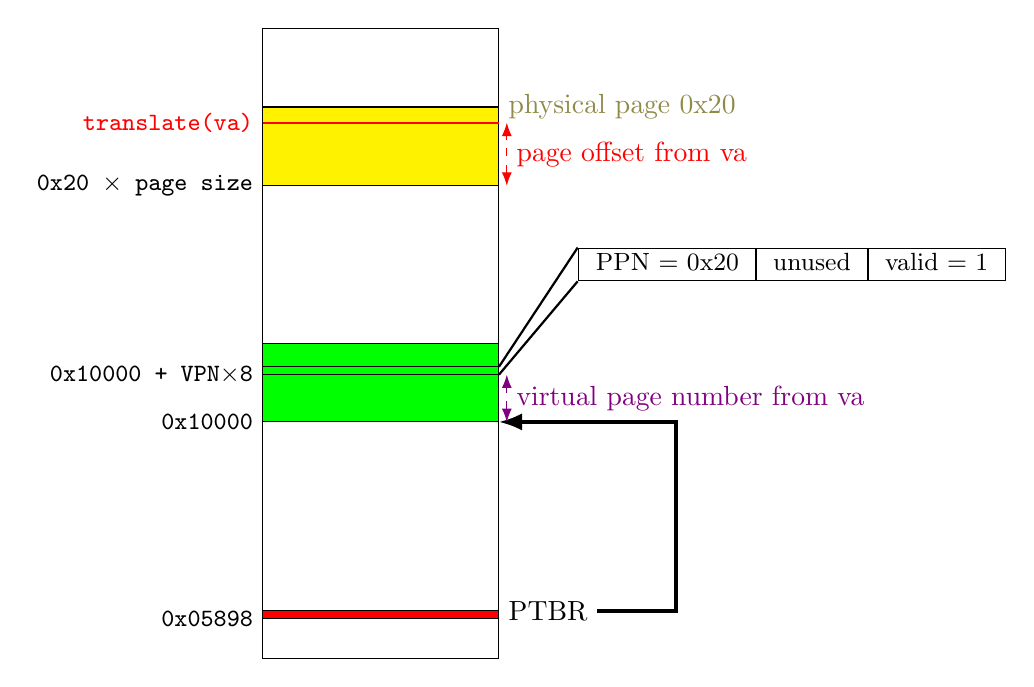
\begin{tikzpicture}
\draw (0, 0) rectangle (3, -8);
\draw[fill=red] (0, -7.5) rectangle (3, -7.4)
    node[right] (ptbr) {PTBR};
\draw[fill=green] (0, -4) rectangle (3, -5);
\draw[-Latex, very thick] (ptbr.east) -- ++(1cm, 0cm) |- (3, -5);
\node[font=\small\tt,anchor=east] at (0, -7.5) {0x05898};
\node[font=\small\tt,anchor=east] at (0, -5) {0x10000};
\node[font=\small\tt,anchor=east] at (0, -4.4) {0x10000 + VPN$\times$8};
\node[font=\small\tt,anchor=east] at (0, -2) {0x20 $\times$ page size};

\draw[Latex-Latex,violet,dashed] (3.1, -5) -- (3.1, -4.4) node[midway,right] {virtual page number from va};
\draw (0, -4.4) rectangle (3, -4.3);
\node[anchor=west,font=\small,inner sep=0mm] (pte) at (4, -3) {
    \begin{tabular}{|l|l|l|} \hline
    PPN = 0x20 & unused & valid = 1 \\ \hline
    \end{tabular}
};
\draw[thick] (3, -4.4) -- (pte.south west);
\draw[thick] (3, -4.3) -- (pte.north west);

\draw[fill=yellow] (0, -2) rectangle (3, -1)
    node[right,yellow!50!black] {physical page 0x20};
\draw[Latex-Latex,red,dashed] (3.1, -2) -- (3.1, -1.2) node[midway, right] {page offset from va};
\draw[thick,red] (0, -1.2) -- (3, -1.2);

\node[red,font=\small\tt,anchor=east] at (0, -1.2) {translate(va)};

\end{tikzpicture}
\end{frame}

\begin{frame}[plain]{first page\_allocate(va) [LEVELS=1]}
\begin{tikzpicture}
\draw (0, 0) rectangle (3, -8);
\draw[fill=red] (0, -7.5) rectangle (3, -7.4)
    node[right] (ptbr) {PTBR};
\begin{visibleenv}<2->
\draw[fill=green] (0, -4) rectangle (3, -5);
\draw[alt=<2>{red},-Latex, very thick] (ptbr.east) -- ++(1cm, 0cm) |- (3, -5);
\end{visibleenv}
\node[font=\small\tt,anchor=east] at (0, -7.5) {0x05898};
\begin{visibleenv}<2->
\node[font=\small\tt,anchor=east] at (0, -5) {NEW0};
\node[font=\small\tt,anchor=east] at (0, -4.4) {NEW0 + VPN$\times$8};
\end{visibleenv}

\draw[Latex-Latex,violet,dashed] (3.1, -5) -- (3.1, -4.4) node[midway,right] {virtual page number from va};
\draw (0, -4.4) rectangle (3, -4.3);
\begin{visibleenv}<2>
\node[anchor=west,font=\small,inner sep=0mm] (pte) at (4, -3) {
    \begin{tabular}{|l|l|l|} \hline
    unused & unused & \myemph<2>{valid = 0} \\ \hline
    \end{tabular}
};
\end{visibleenv}
\begin{visibleenv}<3->
\node[draw=red,anchor=west,font=\small,inner sep=0mm] (pte up) at (4, -3) {
    \begin{tabular}{|l|l|l|} \hline
    PPN = \myemph{NEW1} & unused & \myemph<2>{valid = 1} \\ \hline
    \end{tabular}
};
\end{visibleenv}
\draw[thick] (3, -4.4) -- (pte.south west);
\draw[thick] (3, -4.3) -- (pte.north west);

\begin{visibleenv}<3->
\draw[fill=yellow] (0, -2) rectangle (3, -1);
\node[font=\small\tt,anchor=east] at (0, -2) {\myemph{NEW1} $\times$ page size};
\draw[decorate,decoration={brace,mirror}] (3.1, -2) -- (3.1, -1) node[midway,right] {from posix\_memalign};
\end{visibleenv}
\end{tikzpicture}
\end{frame}

\begin{frame}[plain]{page\_allocate(va) [LEVELS=1]}
\begin{tikzpicture}
\draw (0, 0) rectangle (3, -8);
\draw[fill=red] (0, -7.5) rectangle (3, -7.4)
    node[right] (ptbr) {PTBR};
\draw[fill=green] (0, -4) rectangle (3, -5);
\draw[-Latex, very thick] (ptbr.east) -- ++(1cm, 0cm) |- (3, -5);
\node[font=\small\tt,anchor=east] at (0, -7.5) {0x05898};
\node[font=\small\tt,anchor=east] at (0, -5) {0x10000};
\node[font=\small\tt,anchor=east] at (0, -4.4) {0x10000 + VPN$\times$8};

\draw[Latex-Latex,violet,dashed] (3.1, -5) -- (3.1, -4.4) node[midway,right] {virtual page number from va};
\draw (0, -4.4) rectangle (3, -4.3);
\begin{visibleenv}<1>
\node[anchor=west,font=\small,inner sep=0mm] (pte) at (4, -3) {
    \begin{tabular}{|l|l|l|} \hline
    unused & unused & \myemph<2>{valid = 0} \\ \hline
    \end{tabular}
};
\end{visibleenv}
\begin{visibleenv}<2>
\node[draw=red,anchor=west,font=\small,inner sep=0mm] (pte up) at (4, -3) {
    \begin{tabular}{|l|l|l|} \hline
    PPN = \myemph{NEW} & unused & \myemph<2>{valid = 1} \\ \hline
    \end{tabular}
};
\end{visibleenv}
\draw[thick] (3, -4.4) -- (pte.south west);
\draw[thick] (3, -4.3) -- (pte.north west);

\begin{visibleenv}<2->
\draw[fill=yellow] (0, -2) rectangle (3, -1);
\node[font=\small\tt,anchor=east] at (0, -2) {\myemph{NEW} $\times$ page size};
\draw[decorate,decoration={brace,mirror}] (3.1, -2) -- (3.1, -1) node[midway,right] {from posix\_memalign};
\end{visibleenv}

\end{tikzpicture}
\end{frame}


\usetikzlibrary{arrows.meta,fit,matrix}

\begin{frame}{page table lookup (and translate())}
\begin{tikzpicture}
\tikzset{
    >=Latex,
}
\matrix[tight matrix,anchor=north west,
    nodes={text width=2cm,minimum height=0.6cm},
    column 1/.style={nodes={draw=none,font=\tt,align=right}},
    column 2/.style={nodes={draw,thick,font=\tt,text width=1.2cm,align=center}},
    column 3/.style={nodes={draw,thick,font=\tt, text width=3.5cm}},
    column 4/.style={nodes={draw,thick,font=\tt,visible on=<all:0>, text width=1cm}},
    column 5/.style={nodes={draw,thick,font=\tt,visible on=<all:0>, text width=1cm}},
    row 1/.style={nodes={draw=none,font=\normalfont}},
    ] (pt) at (0, 5) {
    virtual page \# \& valid? \& physical page \# \& read OK? \& write OK? \\
    0\ldots0000 \& |[alias=baseAddr]| 1 \& 01000 \& 1 \& 0 \\
    0\ldots0001 \& 1 \& 11111 \& 1 \& 1 \\
    0\ldots0010 \& 0 \& 00000 \& 0 \& 1 \\
    \ldots \& |[draw=none]| \ldots
           \& |[draw=none]| \ldots
           \& |[draw=none]| \ldots
           \& |[draw=none]| \ldots
           \\
    1\ldots1111 \& 0 \& 01100 \& 1 \& 1 \\
};
\node[alt=<2>{red},font=\tt] (ptbr label) at ([xshift=-6cm]baseAddr.north east) {ptbr};
\draw[alt=<2>{red},ultra thick,dotted,->] (ptbr label) -- (baseAddr.north west);
\node[draw,fill=blue!10] (addrLeft) at (-1, 6.0) {\tt 0\ldots0001};
\node[anchor=west,fill=green!10] (addrRest) at (addrLeft.east) {\tt 1101 0010 \normalfont};
\node[anchor=west] (addrDesc) at (addrRest.east) {--- address from CPU (\texttt{\myemph<1>{va}})};
\draw[->,very thick,draw=blue!50!black] (addrLeft.south) |- ([xshift=0ex]pt-3-1.west);
\draw[->,thick] (pt-6-2.south) |- ++(-1cm,-.25cm) -- ++(0cm,-.25cm) node[below,align=center] {trigger exception if 0?\\(\myemph{return \~~0})};
\draw[->,very thick,draw=blue!50!black] ([xshift=3ex]pt-6-3.south west) |- ++(2cm,-.5cm)
    node[right,fill=blue!10] (newAddrLeft) {\tt 111};
\node[anchor=west,fill=green!10] (newAddrRight) at (newAddrLeft.east) {\tt 1101 0010};
\draw[->,very thick,draw=green!50!black] (addrRest) |- ([xshift=1cm,yshift=.5cm]pt-1-3.north east) -| (newAddrRight);
\node[inner sep=0mm,draw=black,thin,fit=(newAddrLeft) (newAddrRight)] (newAddrBox) {};
\draw[->,very thick] (newAddrBox.south) -- ++(0cm,-.5cm) node[below] {to memory (\texttt{\myemph<1>{translate(va)}})};
\end{tikzpicture}
\end{frame}

\begin{frame}{page table lookup (and allocate)}
\begin{tikzpicture}
\tikzset{
    >=Latex,
}
\begin{visibleenv}<2->
\matrix[tight matrix,anchor=north west,
    nodes={text width=2cm,minimum height=0.6cm},
    column 1/.style={nodes={draw=none,font=\tt,align=right}},
    column 2/.style={nodes={draw,thick,font=\tt,text width=1.2cm,align=center}},
    column 3/.style={nodes={draw,thick,font=\tt, text width=3.5cm}},
    column 4/.style={nodes={draw,thick,font=\tt,visible on=<all:0>, text width=1cm}},
    column 5/.style={nodes={draw,thick,font=\tt,visible on=<all:0>, text width=1cm}},
    row 1/.style={nodes={draw=none,font=\normalfont}},
    ] (pt) at (0, 5) {
    virtual page \# \& valid? \& physical page \# \\%\& read OK? \& write OK? \\
    0\ldots0000 \& |[alias=baseAddr]| 1 \& 01000 \\%\& 1 \& 0 \\
    0\ldots0001 \& |[alt=<2>{fill=red!10}]| 0 \& |[alt=<2>{fill=red!10}]| 00000 \\%\& 0 \& 0 \\
    0\ldots0010 \& 0 \& 00000 \& 0 \& 0 \\
    \ldots \& |[draw=none]| \ldots
           \& |[draw=none]| \ldots
           \\ %\& |[draw=none]| \ldots \& |[draw=none]| \ldots \\
    1\ldots1111 \& 0 \& 01100 \\ %\& 1 \& 1 \\
};
\end{visibleenv}
\node[alt=<1>{red},font=\tt] (ptbr label) at ([xshift=-6cm]baseAddr.north east) {ptbr};
\draw[alt=<1>{red},ultra thick,dotted,->] (ptbr label) -- (baseAddr.north west);
\begin{visibleenv}<1>
\node[fill=white,draw=red,ultra thick] at (pt) {
    allocate\_page(va) --- set ptbr if unset
};
\end{visibleenv}
\node[draw,fill=blue!10] (addrLeft) at (-1, 6.0) {\tt 0\ldots0001};
\node[anchor=west,fill=green!10] (addrRest) at (addrLeft.east) {\tt 1101 0010 \normalfont};
\node[anchor=west] (addrDesc) at (addrRest.east) {--- address from CPU (\texttt{\myemph<1>{va}})};
    \draw[->,very thick,draw=blue!50!black] (addrLeft.south) |- ([xshift=0ex]pt-3-1.west);
    \draw[->,thick] (pt-6-2.south) |- ++(-1cm,-.25cm) -- ++(0cm,-.25cm) node[below,align=center] {trigger exception if 0?\\(\myemph{return \~~0})};
\draw[->,very thick,draw=blue!50!black] ([xshift=3ex]pt-6-3.south west) |- ++(2cm,-.5cm)
    node[right,fill=blue!10] (newAddrLeft) {\tt 111};
    \node[anchor=west,fill=green!10] (newAddrRight) at (newAddrLeft.east) {\tt 1101 0010};
\draw[->,very thick,draw=green!50!black] (addrRest) |- ([xshift=1cm,yshift=.5cm]pt-1-3.north east) -| (newAddrRight);
    \node[inner sep=0mm,draw=black,thin,fit=(newAddrLeft) (newAddrRight)] (newAddrBox) {};
    \draw[->,very thick] (newAddrBox.south) -- ++(0cm,-.5cm) node[below] {to memory (\texttt{\myemph<1>{translate(va)}})};
\begin{visibleenv}<2>
\node[fill=white,align=left,draw=red,ultra thick,anchor=west] at ([xshift=-2cm]pt.east) {
    allocate\_page(va) --- \\set page table entry \\ if unset
};
\end{visibleenv}
\end{tikzpicture}
\end{frame}


\section{handling big page tables}
\subsection{the problem}
\input{../vm/ptSize64A}

\subsection{general options}
\input{../vm/bigPageOptions}

\subsection{two-level page tables}
\input{../vm/twoLevelPtLib}
\input{../vm/twoLevelPT}
\input{../vm/twoLevelPTAlt}

\subsection{more than two levels}
\begin{frame}{multi-level page tables}
    \begin{itemize}
    \item VPN split into pieces for each level of page table
    \vspace{.5cm}
    \item top levels: page table entries point to next page table
        \begin{itemize}
        \item usually using physical page number of next page table
        \end{itemize}
    \item bottom level: page table entry points to destination page
    \vspace{.5cm}
    \item validity checks at \myemph{each level}
    \end{itemize}
\end{frame}


\begin{frame}{note on VPN splitting}
    \begin{itemize}
    \item indexes used for lookup \myemph{parts of the virtual page number}
        \begin{itemize}
        \item (there are not multiple VPNs)
        \end{itemize}
    \end{itemize}
\end{frame}


\subsection{assignment preview}
% FIXME:assignment preview slides
\begin{frame}{assignment}
\end{frame}

\subsection{exercises: multi-level lookup}
% FIXME: \subsubsection{part 0}
% FIXME: \input{../vm/multiSplitExPt0}
\subsubsection{part 2}
\usetikzlibrary{matrix,positioning}

\begin{frame}{2-level splitting}
    \begin{itemize}
    \item 9-bit virtual address 
    \item 6-bit physical address
    \item<2-> \myemph<2>{8-byte pages $\rightarrow$ 3-bit page offset (bottom)}
    \item<2-> 9-bit VA: 6 bit VPN + 3 bit PO
    \item<2-> 6-bit PA: 3 bit PPN + 3 bit PO
    \item<3-> \myemph<3>{1 page page tables w/ 1 byte entry $\rightarrow$ 8 entry PTs}
    \item<4-> \myemph<4>{8 entry page tables $\rightarrow$ 3-bit VPN parts}
    \item<4-> 9-bit VA: 3 bit VPN part 1; 3 bit VPN part 2
    \end{itemize}
\begin{tikzpicture}[overlay,remember picture]
    \coordinate (begin) at ([xshift=-1cm,yshift=-2cm]current page.north east);
    \tikzset{
        page offset/.style={alt=<2>{draw=red,fill=red!10}},
    }
    \begin{scope}[shift={(begin)},x=1.25cm] 
        \draw (-6, 0) rectangle (0, 0.5);
        \node[anchor=south] at (-3, 0.4) {virtual addr};
        \begin{visibleenv}<2-3>
        \draw (-6, 0) rectangle (-2, 0.5) node[midway] {VPN};
        \end{visibleenv}
        \begin{visibleenv}<4->
        \draw (-6, 0) rectangle (-2, 0.5);
            \draw[alt=<4>{red},dotted] (-6, 0) rectangle (-4, 0.5) node[midway,font=\fontsize{11}{12}\selectfont] {VPN pt 1};
            \draw[alt=<4>{red},dotted] (-4, 0) rectangle (-2, 0.5) node[midway,font=\fontsize{11}{12}\selectfont] {VPN pt 2};
        \end{visibleenv}
        \begin{visibleenv}<2->
        \draw[page offset] (-2, 0) rectangle (0, 0.5) node[midway] {page offset};
        \end{visibleenv}
        \begin{scope}[every node/.style={font=\fontsize{10}{11}\selectfont\tt,inner sep=0mm}]
            \node[anchor=north] at (0, 0) {0};
            \node[anchor=north] at (-2, 0) {3};
            \node[anchor=north] at (-4, 0) {6};
            \node[anchor=north] at (-6, 0) {9};
        \end{scope}
        \begin{scope}[yshift=-1.5cm]
            \draw (-4, 0) rectangle (0, 0.5);
            \node[anchor=south] at (-2, 0.4) {physical addr};
            \begin{visibleenv}<2->
            \draw (-4, 0) rectangle (-2, 0.5) node[midway] {PPN};
            \draw[page offset] (-2, 0) rectangle (0, 0.5) node[midway] {page offset};
            \end{visibleenv}
            \begin{scope}[every node/.style={font=\fontsize{10}{11}\selectfont\tt,inner sep=0mm}]
                \node[anchor=north] at (0, 0) {0};
                \node[anchor=north] at (-2, 0) {3};
                \node[anchor=north] at (-4, 0) {6};
            \end{scope}
        \end{scope}
        \begin{visibleenv}<3->
        \begin{scope}[yshift=-4cm]
            \matrix[tight matrix,
                nodes={text width=1cm,font=\small},
                column 1/.style={nodes={text width=0.6cm,draw=none}},
                row 1/.style={nodes={draw=none}},
                label={north:page table \small (either level)},
            ] at (-1, 0){
                ~ \& valid? \& PPN \\
                0 \& ~ \& ~ \\
                1 \& ~ \& ~ \\
                2 \& ~ \& ~ \\
                \ldots \& |[draw=none]|\ldots \& |[draw=none]|\ldots \\
                \myemph<4>{7} \& ~ \& ~ \\
            };
        \end{scope}
        \end{visibleenv}
    \end{scope}
\end{tikzpicture}
\end{frame}

\begin{frame}{2-level example}
\begin{itemize}
\item {}\myemph<1>{9-bit} virtual addresses, 6-bit physical; 8 byte pages, 1 byte PTE
\item page tables 1 page; PTE: 3 bit PPN (MSB), 1 valid bit, 4 unused
\item page table base register {\tt 0x20}; translate virtual address {\tt 0x129}
\end{itemize}
\begin{tikzpicture}
\matrix[tight matrix,anchor=north west,
    nodes={text width=2cm,minimum height=0.5cm,font=\small},
    column 1/.style={nodes={draw=none,font=\small\tt,align=right}},
    column 2/.style={nodes={draw,thick,font=\small\tt,text width=2.6cm,align=left}},
    row 1/.style={nodes={draw=none,font=\small\normalfont}},
    ] (memA)  {
    physical addresses \& bytes \\
    0x00-3 \& 00 11 22 33 \\
    0x04-7 \& 44 55 66 77 \\
    0x08-B \& 88 99 AA BB \\
    0x0C-F \& CC DD EE FF \\
    0x10-3 \& 1A 2A 3A 4A \\
    0x14-7 \& 1B 2B 3B 4B \\
    0x18-B \& 1C 2C 3C 4C \\
    0x1C-F \& 1C 2C 3C 4C \\
};
\matrix[tight matrix,anchor=north west,
    nodes={text width=2cm,minimum height=0.5cm,font=\small},
    column 1/.style={nodes={draw=none,font=\small\tt,align=right}},
    column 2/.style={nodes={draw,thick,font=\small\tt,text width=2.6cm,align=left}},
    row 1/.style={nodes={draw=none,font=\normalfont\small}},
    ] (memB) at ([xshift=0cm]memA.north east) {
    physical addresses \& bytes \\
    0x20-3 \& 00 91 72 13 \\
    0x24-7 \& \maybeEmph<2>{F4} A5 36 07 \\
    0x28-B \& 89 9A AB BC \\
    0x2C-F \& CD DE EF F0 \\
    0x30-3 \& BA \maybeEmph<5>{0A} BA 0A \\
    0x34-7 \& DB 0B DB 0B \\
    0x38-B \& EC 0C EC 0C \\
    0x3C-F \& AC \maybeEmph<3>{DC} DC 0C \\
};
\iftoggle{heldback}{}{
\begin{visibleenv}<2->
\node[right=0cm of memB,align=left,font=\small] {
    {\tt 0x129} = {\tt \myemph<2>{\color<6>{blue}1 00}\myemph<3>{\color<6>{violet}10 1}\myemph<5>{\color<6>{orange}001}} \\
    \texttt{0x20} + {\color<6>{blue}\tt 0x4}~\times 1 = {\tt 0x24} \\
    \textit{PTE 1 value:} \\
    {\tt 0xF4} = {\tt 1111 0100} \\
    PPN {\tt {\color<6>{green} 111}}, valid {\tt 1} \\
    \only<3->{\textit{PTE 2 addr:}} \\
    \only<3->{\texttt{{\color<6>{green} 111} 000} +  \texttt{\myemph<3>{\color<6>{violet} 101}} $\times$ 1 = {\tt 0x3D}}\\
    \only<3->{\textit{PTE 2 value:} {\tt 0xDC}} \\
    \only<4->{PPN {\tt \myemph<4>{\color<6>{red}110}}; valid {\tt 1}} \\
    \only<4->{M[\texttt{\myemph<4>{\color<6>{red}110} \myemph<5>{\color<6>{orange}001}} (\texttt{0x31})] = \texttt{0x0A}}
};
\end{visibleenv}
}
\end{tikzpicture}
\end{frame}

\subsubsection{part 3}
\input{../vm/multiSplitExPt3}
\input{../vm/multiSplitExPt3b}
\subsubsection{part 4}
\input{../vm/multiSplitExPt4}
\subsubsection{part 5}
\input{../vm/multiSplitExPt5}

